\newcommand{\cryptoMinerTagResultsAucTable}{
    \begin{table}[H]
        \centering
        \begin{tabular}{|p{2,8cm}||p{2,8cm} p{2,8cm} p{2,8cm}|}
            \hline
            Crypto-miner Tag & ALOHA & Joint Embedding & Proposed Model \\
            \hline
            AUC-ROC & \textBF{0.639$\pm$0.039} & 0.496$\pm$0.020 & 0.468$\pm$0.025 \\
            \hline
        \end{tabular}
        \caption{AUC-ROC (Area Under Curve) of the different models for the \textbf{Crypto-miner Tag} prediction task. Results were aggregated over \textBF{3} training runs with different weight initializations and minibatch orderings. Best results are shown in \textbf{bold}.} \label{tab:cryptoMinerTag_auc}
    \end{table}
}

\newcommand{\cryptoMinerTagResultsAtFprTable}{
    \begin{center}
        \begin{longtable}[c]{|p{3,2cm}||p{1,8cm} p{1,8cm} p{1,8cm} p{1,8cm} p{1,8cm}|}
            \hline
            Crypto-miner Tag & \multicolumn{5}{c|}{{FPR}} \\
            & $10^{-5}$ & $10^{-4}$ & $10^{-3}$ & $10^{-2}$ & $10^{-1}$ \\
            \hline
            \endfirsthead

            \caption*{\raggedright ...continued from previous page} \\
            \hline
            Crypto-miner Tag & \multicolumn{5}{c|}{\textbf{FPR}} \\
            & $10^{-5}$ & $10^{-4}$ & $10^{-3}$ & $10^{-2}$ & $10^{-1}$ \\
            \hline
            \endhead

            \caption*{\raggedleft ...continued on next page} \\
            \endfoot

            \caption{Mean and standard deviation results (TPR, Accuracy, Recall, Precision and F1-Score) of the different models for the \textbf{Crypto-miner Tag} prediction task at different \textbf{FPR}s (\textit{False Positive Rates}). Results were aggregated over \textBF{3} training runs with different weight initializations and minibatch orderings. Best results are shown in \textbf{bold}. Under \textbf{TPR} results are also presented the percentage reduction in mean detection error and in ROC curve standard deviation introduced by the \textit{Proposed Model} with respect to both \textit{ALOHA} model and \textit{Joint Embedding}.} \label{tab:cryptoMinerTag_results_at_fpr} \\
            \endlastfoot

            \multicolumn{6}{|c|}{\textbf{TPR}} \\
            \hline
            ALOHA & 0.000$\pm$0.000 & 0.000$\pm$0.000 & 0.000$\pm$0.000 & 0.027$\pm$0.000 & \textBF{0.198$\pm$0.025} \\
            Joint Embedding & \textBF{0.009$\pm$0.013} & \textBF{0.009$\pm$0.013} & \textBF{0.009$\pm$0.013} & \textBF{0.036$\pm$0.051} & 0.144$\pm$0.034 \\
            Proposed Model & 0.000$\pm$0.000 & 0.000$\pm$0.000 & 0.000$\pm$0.000 & 0.009$\pm$0.013 & 0.072$\pm$0.034 \\
            \hline
            Error Reduction wrt \newline ALOHA & 0.0\% & 0.0\% & 0.0\% & -1.8\% & -15.7\% \\
            Error Reduction wrt \newline Joint Embedding & -0.9\% & -0.9\% & -0.9\% & -2.8\% & -8.4\% \\
            \hline
            Std Reduction wrt \newline ALOHA & 0.0\% & 0.0\% & 0.0\% & 0.0\% & -36.0\% \\
            Std Reduction wrt \newline Joint Embedding & 100.0\% & 100.0\% & 100.0\% & 74.5\% & 0.0\% \\
            \hline
            \multicolumn{6}{|c|}{\textbf{Accuracy}} \\
            \hline
            ALOHA & \textBF{0.985$\pm$0.000} & \textBF{0.985$\pm$0.000} & 0.984$\pm$0.000 & 0.977$\pm$0.001 & 0.892$\pm$0.001 \\
            Joint Embedding & \textBF{0.985$\pm$0.000} & \textBF{0.985$\pm$0.000} & \textBF{0.985$\pm$0.000} & 0.982$\pm$0.002 & 0.891$\pm$0.003 \\
            Proposed Model & \textBF{0.985$\pm$0.000} & \textBF{0.985$\pm$0.000} & 0.984$\pm$0.000 & \textBF{0.983$\pm$0.002} & \textBF{0.894$\pm$0.009} \\
            \hline
            \multicolumn{6}{|c|}{\textbf{Recall}} \\
            \hline
            ALOHA & 0.000$\pm$0.000 & 0.000$\pm$0.000 & 0.000$\pm$0.000 & 0.027$\pm$0.000 & \textBF{0.198$\pm$0.025} \\
            Joint Embedding & \textBF{0.009$\pm$0.013} & \textBF{0.009$\pm$0.013} & \textBF{0.009$\pm$0.013} & \textBF{0.036$\pm$0.051} & 0.144$\pm$0.034 \\
            Proposed Model & 0.000$\pm$0.000 & 0.000$\pm$0.000 & 0.000$\pm$0.000 & 0.009$\pm$0.013 & 0.072$\pm$0.034 \\
            \hline
            \multicolumn{6}{|c|}{\textbf{Precision}} \\
            \hline
            ALOHA & \textBF{1.000$\pm$0.000} & \textBF{1.000$\pm$0.000} & 0.000$\pm$0.000 & 0.048$\pm$0.008 & \textBF{0.030$\pm$0.004} \\
            Joint Embedding & \textBF{1.000$\pm$0.000} & \textBF{1.000$\pm$0.000} & \textBF{0.333$\pm$0.471} & \textBF{0.067$\pm$0.094} & 0.022$\pm$0.006 \\
            Proposed Model & \textBF{1.000$\pm$0.000} & \textBF{1.000$\pm$0.000} & 0.000$\pm$0.000 & 0.022$\pm$0.031 & 0.011$\pm$0.005 \\
            \hline
            \multicolumn{6}{|c|}{\textbf{F1 Score}} \\
            \hline
            ALOHA & 0.000$\pm$0.000 & 0.000$\pm$0.000 & 0.000$\pm$0.000 & 0.034$\pm$0.002 & \textBF{0.052$\pm$0.007} \\
            Joint Embedding & \textBF{0.018$\pm$0.025} & \textBF{0.018$\pm$0.025} & \textBF{0.018$\pm$0.025} & \textBF{0.047$\pm$0.066} & 0.039$\pm$0.010 \\
            Proposed Model & 0.000$\pm$0.000 & 0.000$\pm$0.000 & 0.000$\pm$0.000 & 0.013$\pm$0.018 & 0.019$\pm$0.008 \\
            \hline
        \end{longtable}
    \end{center}
}

\newcommand{\cryptoMinerTagResultsSummaryTable}{
    \begin{table}[H]
        \centering
        \begin{tabular}{|p{3,2cm}||p{1,8cm} p{1,8cm} p{1,8cm} p{1,8cm} p{1,8cm}|}
            \hline
            \multicolumn{6}{|c|}{Crypto-miner Tag (at FPR $=1\%$)} \\
            \hline
            Model & TPR & Accuracy & Precision & Recall & F1 score \\
            \hline
            ALOHA & 0.027$\pm$0.000 & 0.977$\pm$0.001 & 0.048$\pm$0.008 & 0.027$\pm$0.000 & 0.034$\pm$0.002 \\
            Joint Embedding & \textBF{0.036$\pm$0.051} & 0.982$\pm$0.002 & \textBF{0.067$\pm$0.094} & \textBF{0.036$\pm$0.051} & \textBF{0.047$\pm$0.066} \\
            Proposed Model & 0.009$\pm$0.013 & \textBF{0.983$\pm$0.002} & 0.022$\pm$0.031 & 0.009$\pm$0.013 & 0.013$\pm$0.018 \\
            \hline
        \end{tabular}
        \caption{Summary of the mean and standard deviation results of the different models for the \textbf{Crypto-miner Tag} prediction task at \textbf{FPR} $=1\%$. Results were aggregated over \textBF{3} training runs with different weight initializations and minibatch orderings. Best results are shown in \textbf{bold}.} \label{tab:cryptoMinerTag_result_summary}
    \end{table}
}

\newcommand{\cryptoMinerTagRocAloha}{
    \begin{figure}[H]
        \centering
        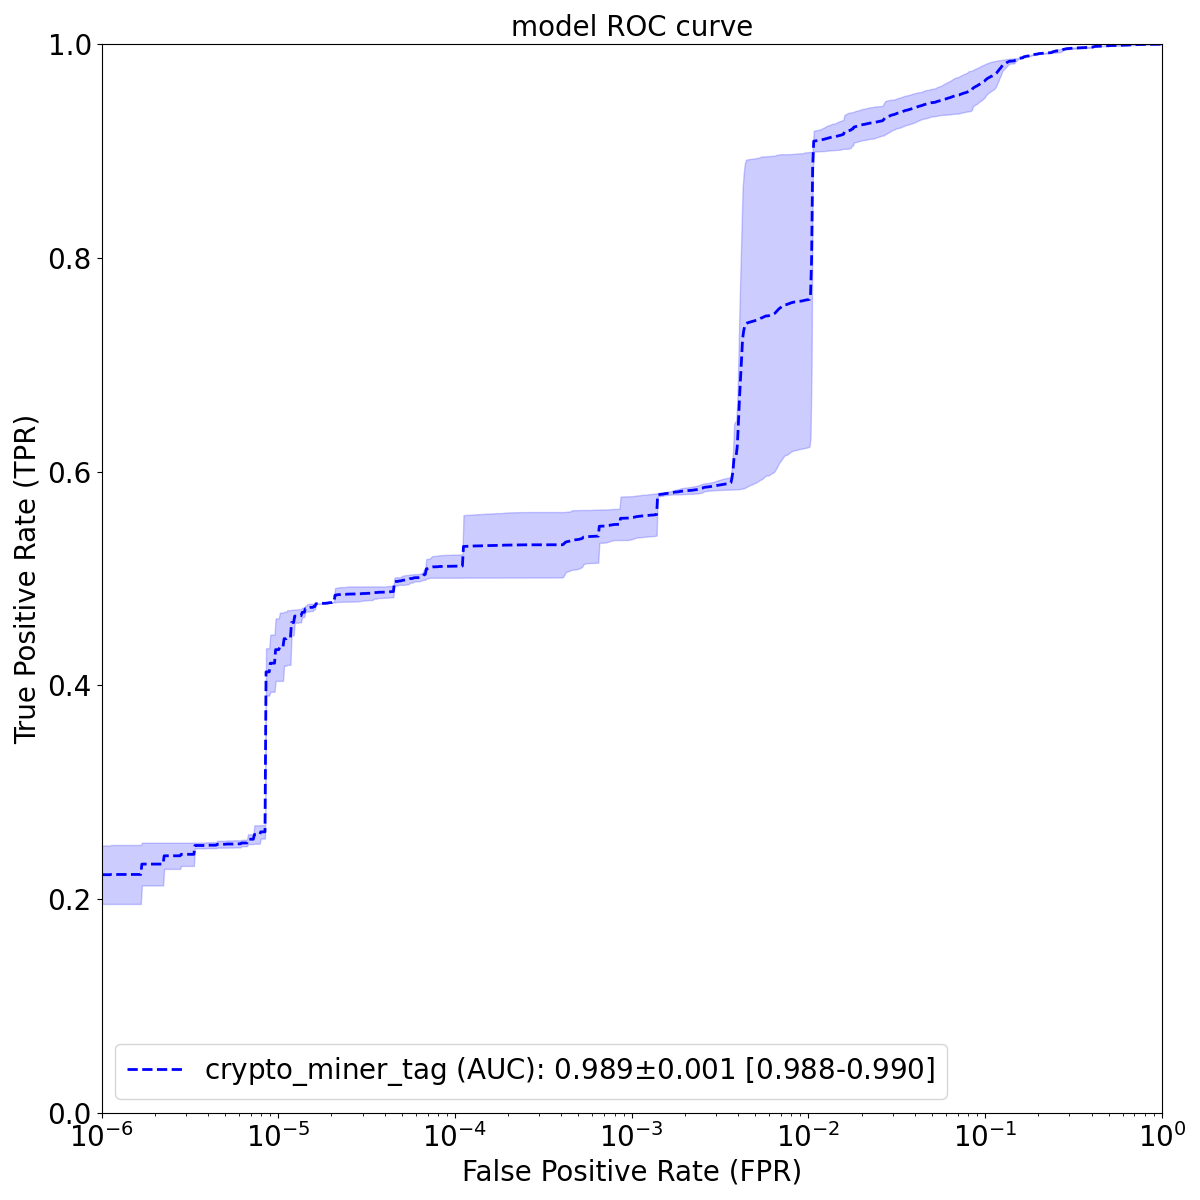
\includegraphics[width=0.8\textwidth]{./results/crypto_miner_tag_roc_aloha.png}
        \vspace*{-1cm}
        \caption{ROC curve and AUC statistics of \textBF{ALOHA} model for the \textbf{Crypto-miner Tag}. The line represents the \textit{mean} TPR at a given FPR, while the shaded region represents the \textit{standard deviation}. Statistics were computed over \textBF{3} training runs, each with random parameter initialization.}
        \label{fig:cryptoMinerTagRocAloha}
    \end{figure}
}

\newcommand{\cryptoMinerTagRocJointEmbedding}{
    \begin{figure}[H]
        \centering
        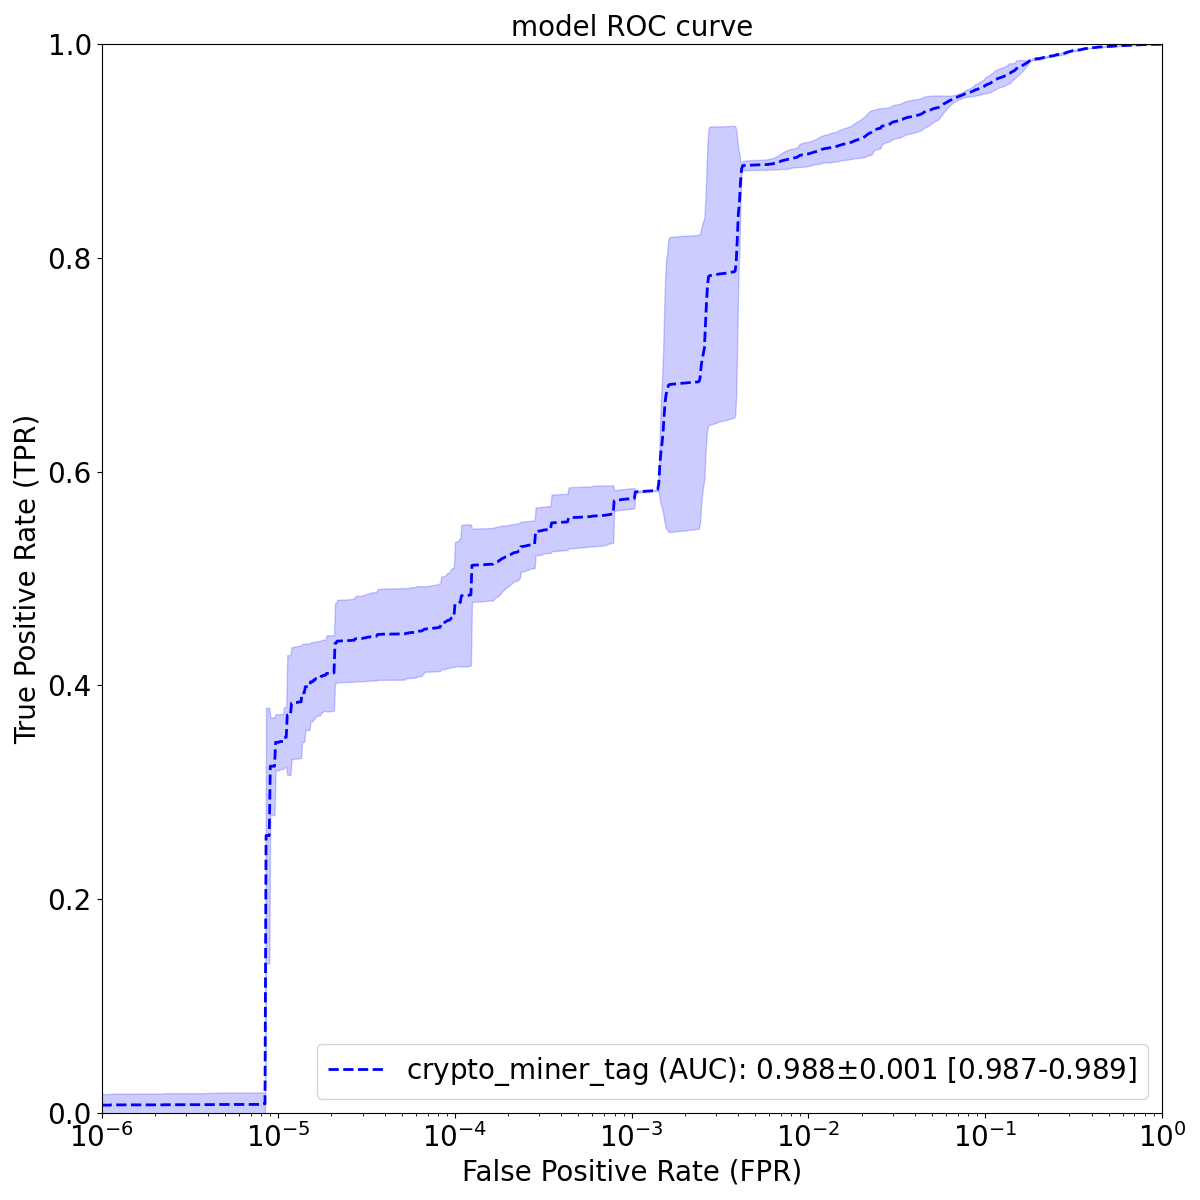
\includegraphics[width=0.8\textwidth]{./results/crypto_miner_tag_roc_jointEmbedding.png}
        \vspace*{-1cm}
        \caption{ROC curve and AUC statistics of \textBF{Joint Embedding} model for the \textbf{Crypto-miner Tag}. The line represents the \textit{mean} TPR at a given FPR, while the shaded region represents the \textit{standard deviation}. Statistics were computed over \textBF{3} training runs, each with random parameter initialization.}
        \label{fig:cryptoMinerTagRocJointEmbedding}
    \end{figure}
}

\newcommand{\cryptoMinerTagRocProposedMethod}{
    \begin{figure}[H]
        \centering
        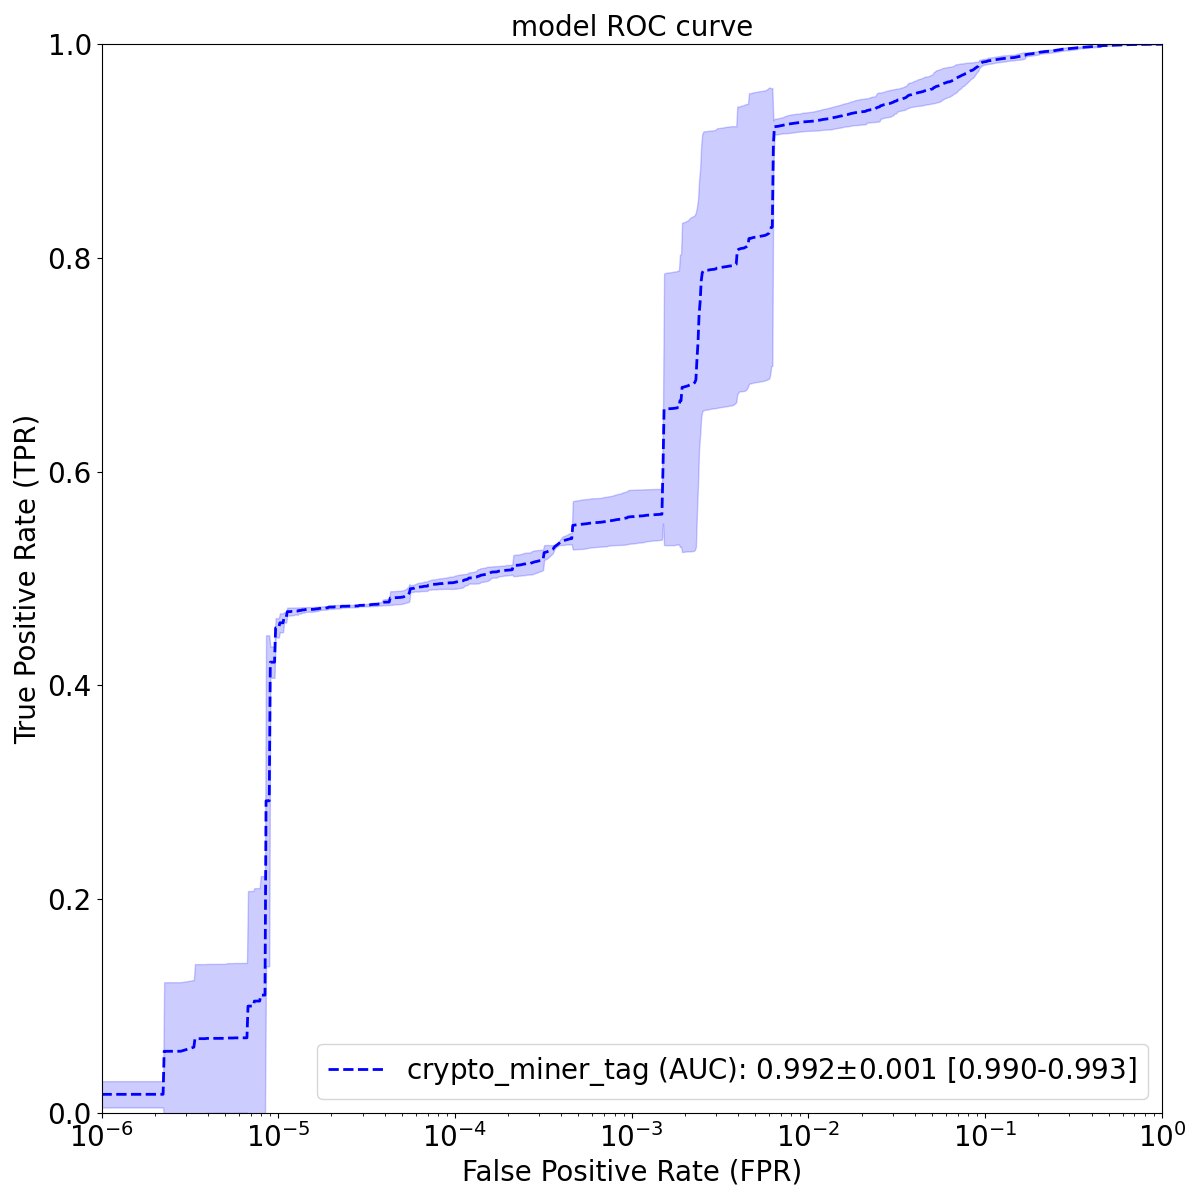
\includegraphics[width=0.8\textwidth]{./results/crypto_miner_tag_roc_proposedModel.png}
        \vspace*{-1cm}
        \caption{ROC curve and AUC statistics of \textBF{Proposed Model} for the \textbf{Crypto-miner Tag}. The line represents the \textit{mean} TPR at a given FPR, while the shaded region represents the \textit{standard deviation}. Statistics were computed over \textBF{3} training runs, each with random parameter initialization.}
        \label{fig:cryptoMinerTagRocProposedModel}
    \end{figure}
}
